\section{Cloud Computing}\label{sec:cloud-computing}

\subsection{What is}\label{subsec:what-is-cloud-computin}

Cloud computing is the \textbf{on-demand delivery} of it resources (database storage, compute power, etc), which you can access and \textbf{provision the right type and size of computing} \textbf{almost instantly} and have a \textbf{pay-as-you-go} pricing.

\subsection{Deployment Models of the Cloud}\label{subsec:deployment-models-of-the-cloud}

\begin{enumerate}
	\item \textbf{Private:}
	\begin{itemize}
		\item Complete control, meet specific business needs
		\item Used by single organization
		\item Cloud owned by third-party
	\end{itemize}
  	\item \textbf{Public:}
  	\begin{itemize}
  		\item Cloud resources owned and operated by third-party.
  	\end{itemize}
  	\item \textbf{Hybrid:}
  	\begin{itemize}
  		\item Keep the control of some servers and extend  some capabilities to the Cloud
  	\end{itemize}
\end{enumerate}

\subsection{Five Characteristics of Cloud Computing (Amazon POV)}\label{subsec:five-characteristics-of-cloud-computing-(amazon-pov)}

\begin{itemize}
	\item \textbf{On-demand self service:} Users can provide it resources without human interaction.
	\item \textbf{Broad network access:} Can access the AWS panel from the internet.
	\item \textbf{Multi-tenancy and resource pooling:} Multiple users share the same physical resources yet their it resources are isolated with security and privacy.
	\item \textbf{Rapid elasticity and scalability:} Automatically and quickly add or remove it resources.
	\item \textbf{Measured service:} Usage is measured and you pay what you use.
\end{itemize}

\subsection{Advantages of Cloud Computing}\label{subsec:advantages-of-cloud-computing}

\begin{itemize}
	\item \textbf{Trade CAPEX for OPEX:} Pay on-demand don't own hardware.
	\item \textbf{Benefit from economies of scale:} If more people use AWS, AWS will acquire more hardware and become more efficient, then the pricing goes lower.
	\item \textbf{Use what you need:} Scale based on actual usage measure.
	\item \textbf{Increase speed and agility:} Instance resources almost immediately.
	\item \textbf{Globality:} Instance IT resources in many geographical locations.
\end{itemize}

\subsection{Problems solved by the Cloud (Business with IT needs POV)}\label{subsec:problems-solved-by-the-cloud-(business-with-it-needs-pov)}
\begin{itemize}
	\item \textbf{Flexibility:} Add, remove and change IT resources when needed.
	\item \textbf{Cost-effectiveness:} Pay as-you-go.
	\item \textbf{Scalability:} Increase IT resources when receiving larger loads.
	\item \textbf{Elasticity:} Scale-in and scale-out when needed.
	\item \textbf{High-availability and` Fault-tolerant:} You gotta trust AWS.
	\item \textbf{Agility:} Quick development process, test and launch software applications.
\end{itemize}

\subsection{AWS Global Infrastructure}\label{subsec:aws-global-infrastructure}
\begin{figure}[h]
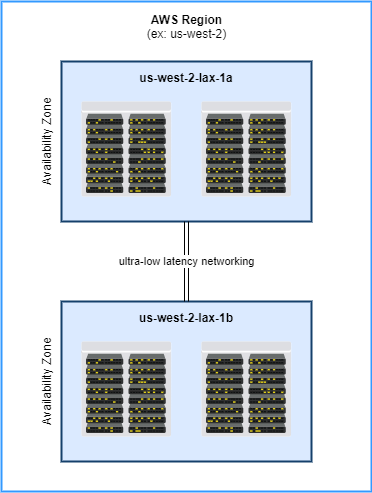
\includegraphics[scale=0.5]{cloud-computing/regions}
\centering\label{fig:aws-global-infrastructure}
\end{figure}

